% CVPR-style template
\documentclass[10pt,twocolumn,letterpaper]{article}

\usepackage[pagenumbers]{cvpr}
\usepackage{graphicx}
\usepackage{subcaption}
\usepackage{amsmath}
\usepackage{amssymb}
\usepackage{booktabs}
\usepackage{array}
\usepackage{tabularx}
\usepackage[dvipsnames]{xcolor}
\usepackage{xeCJK}
\setCJKmainfont{Noto Serif CJK TC}
\usepackage[pagebackref,breaklinks,colorlinks]{hyperref}
\usepackage[capitalize]{cleveref}
\crefname{section}{Sec.}{Secs.}
\Crefname{section}{Section}{Sections}
\crefname{table}{Tab.}{Tabs.}
\Crefname{table}{Table}{Tables}

\begin{document}

\title{\LARGE HW3: Instance Segmentation Report \\[0.5em] \large Visual Recognition using Deep Learning, NYCU}
\author{朱驛庭, 111550093}
\maketitle

\section{Introduction}
\label{sec:intro}

This work tackles the HW3 colored medical image instance segmentation task. The dataset contains 209 training images and 101 test images. Each image may contain four cell categories, and each non-zero connected instance id in \texttt{class1.tif}--\texttt{class4.tif} is an object mask. The evaluation metric is AP$_{50}$ for instance segmentation, so the most important factors are recall, classification correctness, and avoiding duplicate instances; extremely precise mask boundaries are less critical than in AP@[.50:.95].

The dataset is small but highly dense and imbalanced. The two frequent classes contain 14{,}537 and 15{,}653 instances, while class3 and class4 contain only 630 and 587 instances. Some images contain more than 700 cells, and image sizes range from tiny crops to images over 2000 pixels. These properties led us to use a Mask R-CNN-family method with small anchors, a high detection cap, multi-scale augmentation, and memory-safe streaming test-time augmentation (TTA).

The final best public submission is \textbf{0.5624 AP$_{50}$}, obtained by a TorchVision Mask R-CNN ResNet-50-FPN model with vertical/horizontal flip TTA and multi-scale mask fusion. This corresponds to public leaderboard rank 25 under team name \texttt{chueating}. The project repository is available at \url{https://github.com/ChuEating1005/VRDL/tree/main/HW3}.

\section{Method}
\label{sec:method}

\subsection{Model}
We use Mask R-CNN~\cite{he2017mask} with a ResNet-50~\cite{he2016resnet} backbone and Feature Pyramid Network (FPN)~\cite{lin2017fpn}. ImageNet pretrained weights are used for the backbone only, satisfying the homework constraint. The model has \textbf{43.72M trainable parameters}, below the 200M parameter limit.

The key components are as follows. The \textbf{backbone} is ResNet-50, which extracts convolutional features at multiple spatial resolutions. The \textbf{neck} is FPN, which builds a top-down feature pyramid so that small cells can be detected from high-resolution features while larger cells still use semantically strong deep features. The \textbf{RPN head} proposes candidate boxes on every FPN level using small anchors. The \textbf{RoI box head} classifies proposals into four cell classes and refines their bounding boxes. The \textbf{mask head} predicts a binary mask for each positive RoI with the standard BCE mask loss. The final submission converts the per-instance mask logits into binary masks and then COCO RLE.

The baseline configuration is designed for dense small objects:
\begin{itemize}
  \item small anchors, with pyramid anchor sizes starting at 16 pixels;
  \item \texttt{detections\_per\_img=1000}, because a single test image can contain hundreds of cells;
  \item low box score threshold 0.05 to preserve recall for AP$_{50}$;
  \item model-side resize cap \texttt{min\_size=512}, \texttt{max\_size=1024} to avoid dense-mask OOM.
\end{itemize}

We also implemented several ablation switches: ResNet-101, ConvNeXt-Tiny~\cite{liu2022convnet}, PAFPN/PANet-style bottom-up path aggregation~\cite{liu2018path}, BCE+Dice mask loss, Copy-Paste~\cite{ghiasi2021simple}, and rare-class weighted sampling.

These modifications were not only hyper-parameter tuning. They change model components or training data distribution: PAFPN changes the neck topology, Dice changes the mask optimization objective, Copy-Paste changes the instance-level data distribution, rare-class sampling changes image sampling frequency, and 5-fold ensembling changes the inference model set.

\subsection{Data Processing and Augmentation}
TIFF images are loaded as RGB by dropping the constant alpha channel. For masks, each unique non-zero value is treated as one instance. Training augmentations include longest-side resize to 1024, random scale in [0.6, 1.6], another longest-side cap, horizontal/vertical flips, random 90-degree rotations, brightness/contrast, HSV jitter, CLAHE, and light blur.

Because class3 and class4 are rare, we tested two imbalance strategies. The first is binary rare-class weighted sampling: images containing class3 or class4 receive sample weight $1+t$ with $t=1.0$. The second is rare-class Copy-Paste, where class3/class4 instances are pasted onto the same canvas with probability 0.3. Both are intuitive, but both hurt public score in our experiments (see \cref{sec:negative}).

\subsection{Training}
The main baseline uses SGD with momentum 0.9, learning rate 0.0025, weight decay $10^{-4}$, batch size 2, and 20 epochs. The trainable backbone layers are set to 3, and the RPN train/test pre-NMS and post-NMS proposal caps are 1000/500. The RoI box batch size per image is 256. We later trained a 30-epoch version, which achieved better validation AP$_{50}$ but lower public score, suggesting validation overfitting on the small split. We also implemented an AdamW~\cite{loshchilov2019adamw} + cosine schedule baseline inspired by prior solutions, but it was not selected as the final submission path.

All runs are logged to Weights \& Biases under project \texttt{vrdl-hw3}. Validation uses COCO-style mask AP and additionally logs per-class AP$_{50}$.

\subsection{Streaming TTA and Submission Format}
The largest gain came from inference. We use flip TTA over identity, horizontal flip, vertical flip, and horizontal+vertical flip. The best run also uses multi-scale TTA with scales 0.83, 1.0, and 1.17. For each augmented prediction, boxes and masks are mapped back to original image coordinates.

Naively accumulating all augmented outputs on GPU causes OOM because TorchVision pastes predicted masks back to full image resolution. Therefore TTA is performed in a streaming manner: after each augmented forward pass, predictions are moved to CPU candidates, GPU tensors are deleted, and CUDA cache is cleared. The final fusion is done on CPU.

We tested two TTA fusion modes. NMS fusion keeps the highest-scoring box per class after box NMS. Mask fusion groups predictions by box IoU, averages decoded binary masks weighted by confidence, thresholds the averaged mask, and converts it back to COCO RLE. Final records use the required COCO schema: 1-indexed \texttt{category\_id}, \texttt{bbox=[x,y,w,h]}, and RLE \texttt{counts} encoded as strings.

\section{Experiments}
\label{sec:experiments}

\subsection{Submission Results}
\cref{tab:submissions} summarizes all public submissions and important local experiments. The best result is 0.5624 AP$_{50}$ from the baseline checkpoint plus vhflip multi-scale TTA.

\begin{figure}[t]
  \centering
  
\includegraphics[width=\linewidth]{assets/leaderboard_screenshot.png}
  \caption{Final public leaderboard entry. The best submission reaches 0.5624 AP$_{50}$ and rank 25.}
  \label{fig:leaderboard}
\end{figure}

\begin{table*}[t]
  \centering
  \scriptsize
  \setlength{\tabcolsep}{3pt}
  \begin{tabularx}{\textwidth}{p{0.28\textwidth}p{0.18\textwidth}cXc}
    \toprule
    \textbf{Run} & \textbf{Main change} & \textbf{Epoch} & \textbf{Inference} & \textbf{Public AP$_{50}$} \\ \midrule
    baseline-v1 & R50-FPN Mask R-CNN & 20 & none & 0.5134 \\
    baseline-v1-vhflip-nms & same ckpt & 20 & vhflip + NMS fusion & 0.5539 \\
    baseline-v1-vhflip-mask & same ckpt & 20 & vhflip + mask fusion & 0.5525 \\
    baseline-v1-vhflip-nms-ms & same ckpt & 20 & vhflip + scales 0.83/1.0/1.17 + NMS fusion & \textbf{0.5624} \\
    baseline-v1-ep30-vhflip-nms-ms & longer training & 30 & vhflip + scales 0.83/1.0/1.17 + NMS fusion & 0.5558 \\
    r50-pafpn-vhflip-nms & PAFPN neck & 30 & vhflip + NMS fusion & 0.5356 \\
    r50-pafpn-vhflip-nms-ms & PAFPN neck & 30 & vhflip + scales 0.83/1.0/1.17 + NMS fusion & 0.5480 \\
    r50-cp-vhflip-nms-ms & Copy-Paste & 30 & vhflip + scales 0.83/1.0/1.17 + NMS fusion & 0.5545 \\
    r50-rfs-cp-vhflip-nms-ms & RFS + Copy-Paste & 30 & vhflip + scales 0.83/1.0/1.17 + NMS fusion & 0.5370 \\
    r50-rfs-vhflip-nms-ms & RFS & 30 & vhflip + scales 0.83/1.0/1.17 + NMS fusion & 0.5312 \\
    r50-cp-ep20-tta & Copy-Paste & 20 & vhflip + scales 0.83/1.0/1.17 + NMS fusion & 0.5410 \\
    baseline-v1-tta-det300 & lower detection & 20 & vhflip + scales 0.83/1.0/1.17 + NMS fusion & 0.5356 \\
    baseline-v1-ep20-fold0-tta & one CV fold & 20 & vhflip + scales 0.83/1.0/1.17 + mask fusion & 0.4573 \\
    baseline-v1-ep20-5fold-tta & fused per-fold JSONs & 20 & post-hoc JSON mask fusion & 0.5078 \\
    baseline-v1-ep20-5ckpt-direct-tta & direct 5-ckpt ensemble & 20 & model$\times$TTA raw fusion & 0.5042 \\
    \bottomrule
  \end{tabularx}
  \caption{Public leaderboard AP$_{50}$ summary. The strongest improvement is TTA, not a heavier architecture.}
  \label{tab:submissions}
\end{table*}

\subsection{Effect of TTA}
The most important finding is that TTA dramatically improves AP$_{50}$. Starting from the baseline score 0.5134, adding vertical/horizontal flip TTA and NMS raises performance to 0.5539 (+4.05 percentage points). Adding multi-scale inference further raises performance to 0.5624. This is consistent with the dataset: cells appear at diverse sizes, and AP$_{50}$ rewards recovering more true instances.

Mask fusion and NMS fusion are close at single scale: 0.5525 vs. 0.5539. Multi-scale mask fusion gives the final best result, but its downside is inference cost. The final TTA setting requires 12 forward passes per image and must be streamed to prevent VRAM overflow.

\subsection{Validation/Public Gap}
The 30-epoch baseline achieved higher validation AP$_{50}$ (0.52799 vs. 0.49902 for the 20-epoch baseline) but worse public AP$_{50}$ (0.5558 vs. 0.5624). This indicates that the random validation split is not fully representative of the public test distribution. Therefore, after this point, public submissions were treated as the primary selection signal, while validation was used only for sanity checking.

\begin{figure*}[t]
  \centering
  \begin{subfigure}[t]{0.32\linewidth}
    
\includegraphics[width=\linewidth]{assets/epoch/val_ap50.png}
    \caption{Epoch ablation. Validation improves from epoch 20 to 30, but public score drops.}
  \end{subfigure}
  \hfill
  \begin{subfigure}[t]{0.32\linewidth}
    
\includegraphics[width=\linewidth]{assets/backbone-beck/val_ap50.png}
    \caption{Backbone/neck ablation. R50-PAFPN looks competitive on validation but not on public test.}
  \end{subfigure}
  \hfill
  \begin{subfigure}[t]{0.32\linewidth}
    
\includegraphics[width=\linewidth]{assets/rfs-cp/val_ap50.png}
    \caption{RFS/Copy-Paste ablation. Validation gains do not transfer to public AP$_{50}$.}
  \end{subfigure}
  \caption{Representative Weights \& Biases validation curves. These curves explain why validation-only model selection was unreliable for this small dataset.}
  \label{fig:val_curves}
\end{figure*}

\subsection{Fold and Per-Class Variance}
The 5-fold experiment revealed a stronger issue than ordinary overall fold variance: the best fold differs by class. As shown in \cref{fig:fold_curves}, class1 is best on fold2, class2 on fold3, class3 on fold0, and class4 on fold4. The final AP$_{50}$ spread is large: roughly 0.14 for class1, 0.09 for class2, 0.17 for class3, and 0.28 for class4. This means each fold learns a different class balance, so a single validation fold is a noisy proxy for the public test set.

\begin{figure*}[t]
  \centering
  \begin{subfigure}[t]{0.32\linewidth}
    
\includegraphics[width=\linewidth]{assets/5-fold/train_loss.png}
    \caption{Training loss.}
  \end{subfigure}
  \hfill
  \begin{subfigure}[t]{0.32\linewidth}
    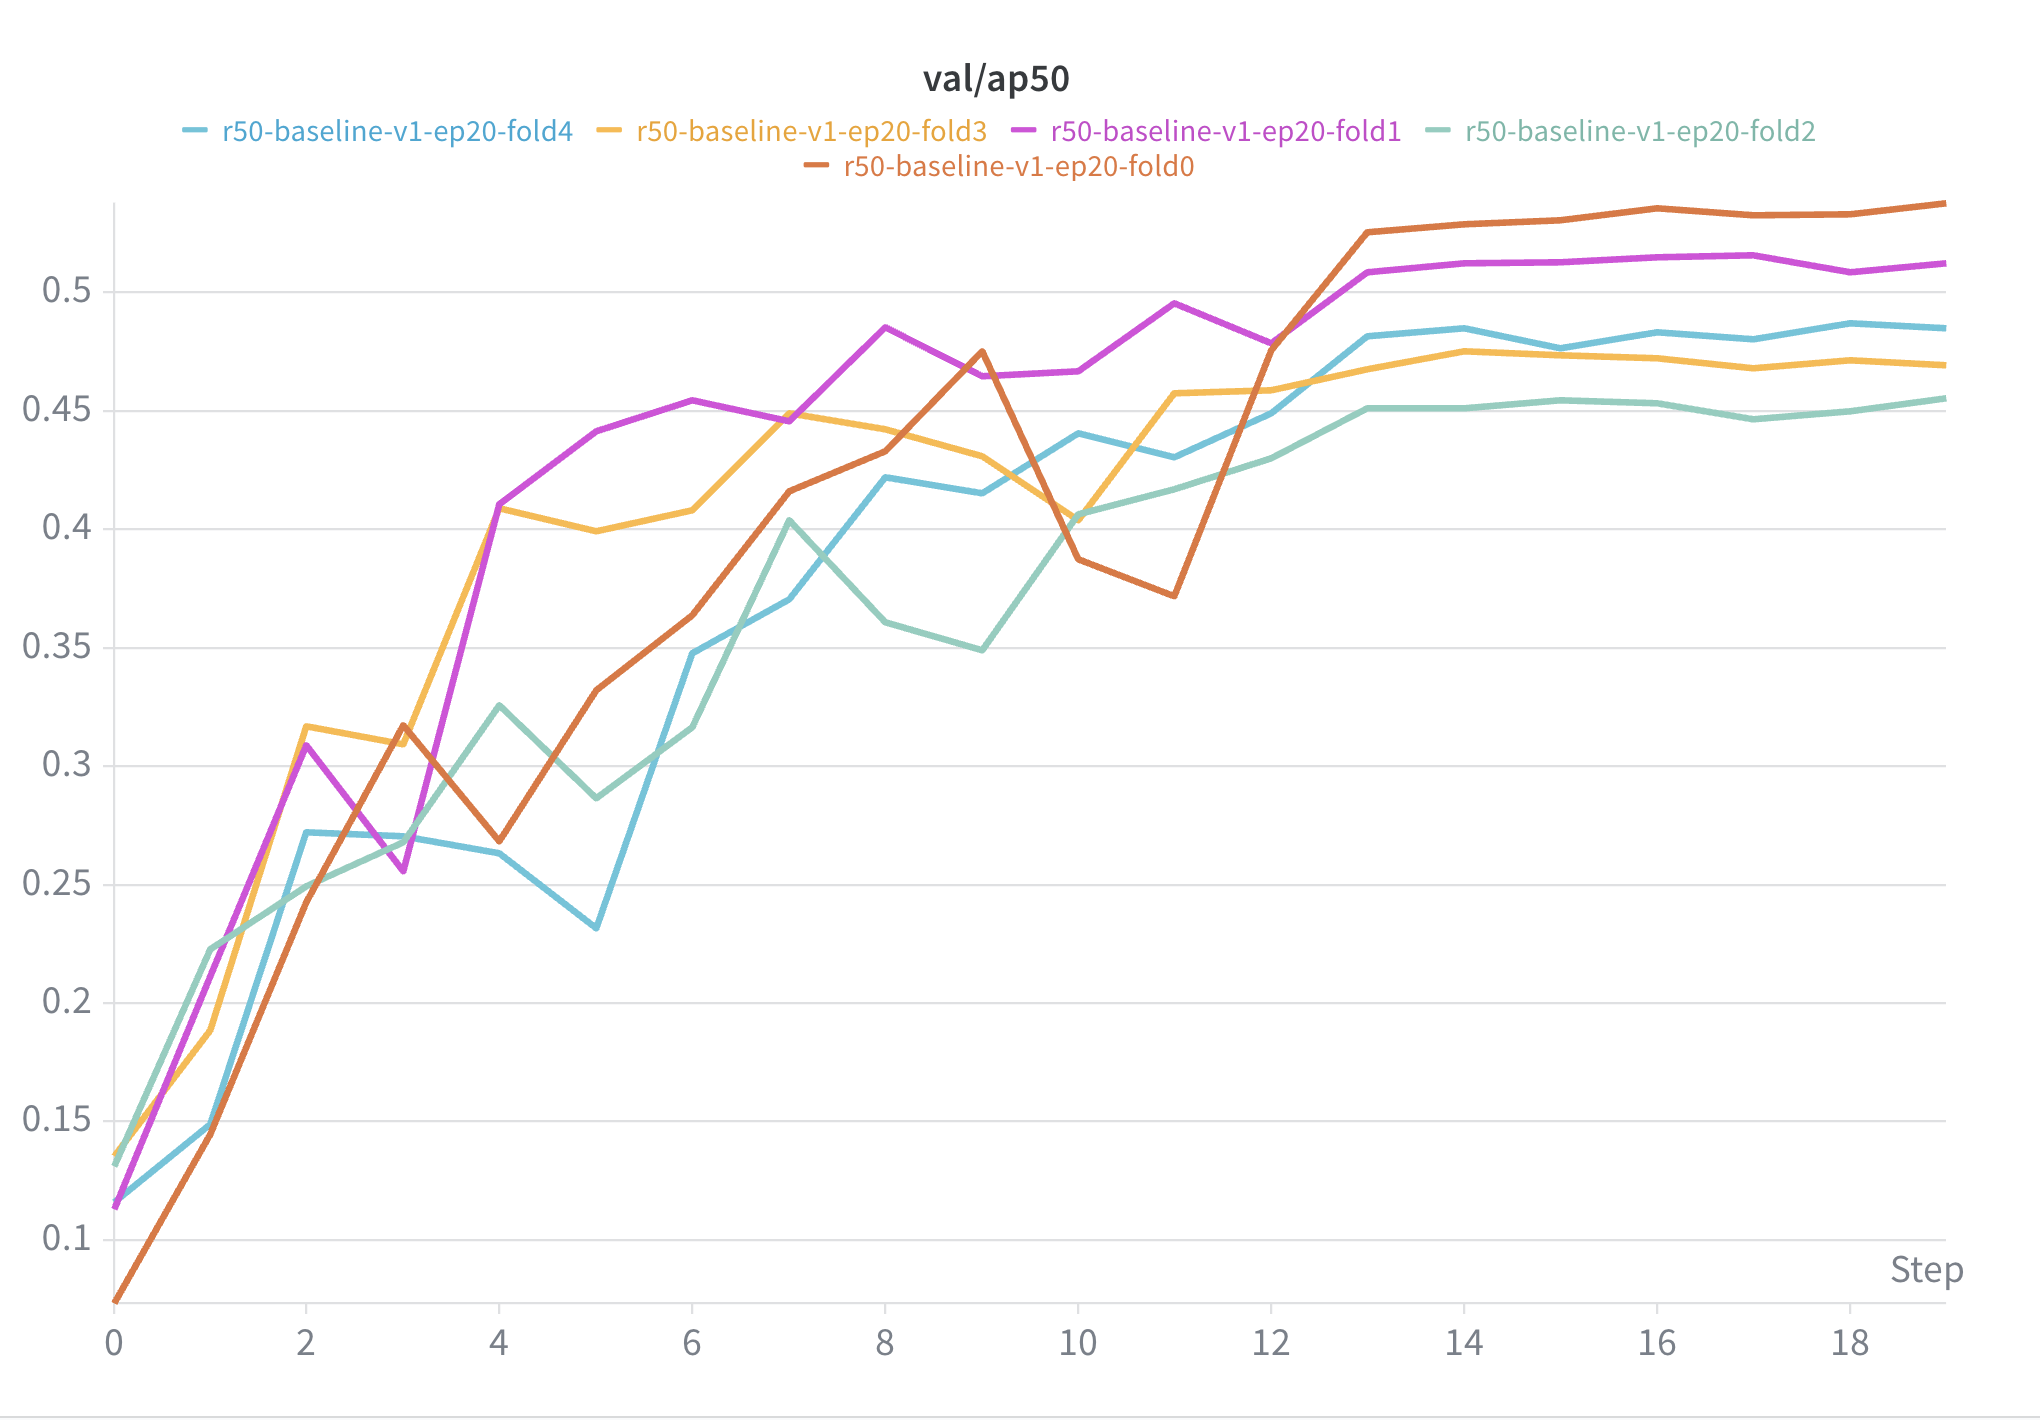
\includegraphics[width=\linewidth]{assets/5-fold/val_ap50.png}
    \caption{Overall fold AP$_{50}$.}
  \end{subfigure}
  \hfill
  \begin{subfigure}[t]{0.32\linewidth}
    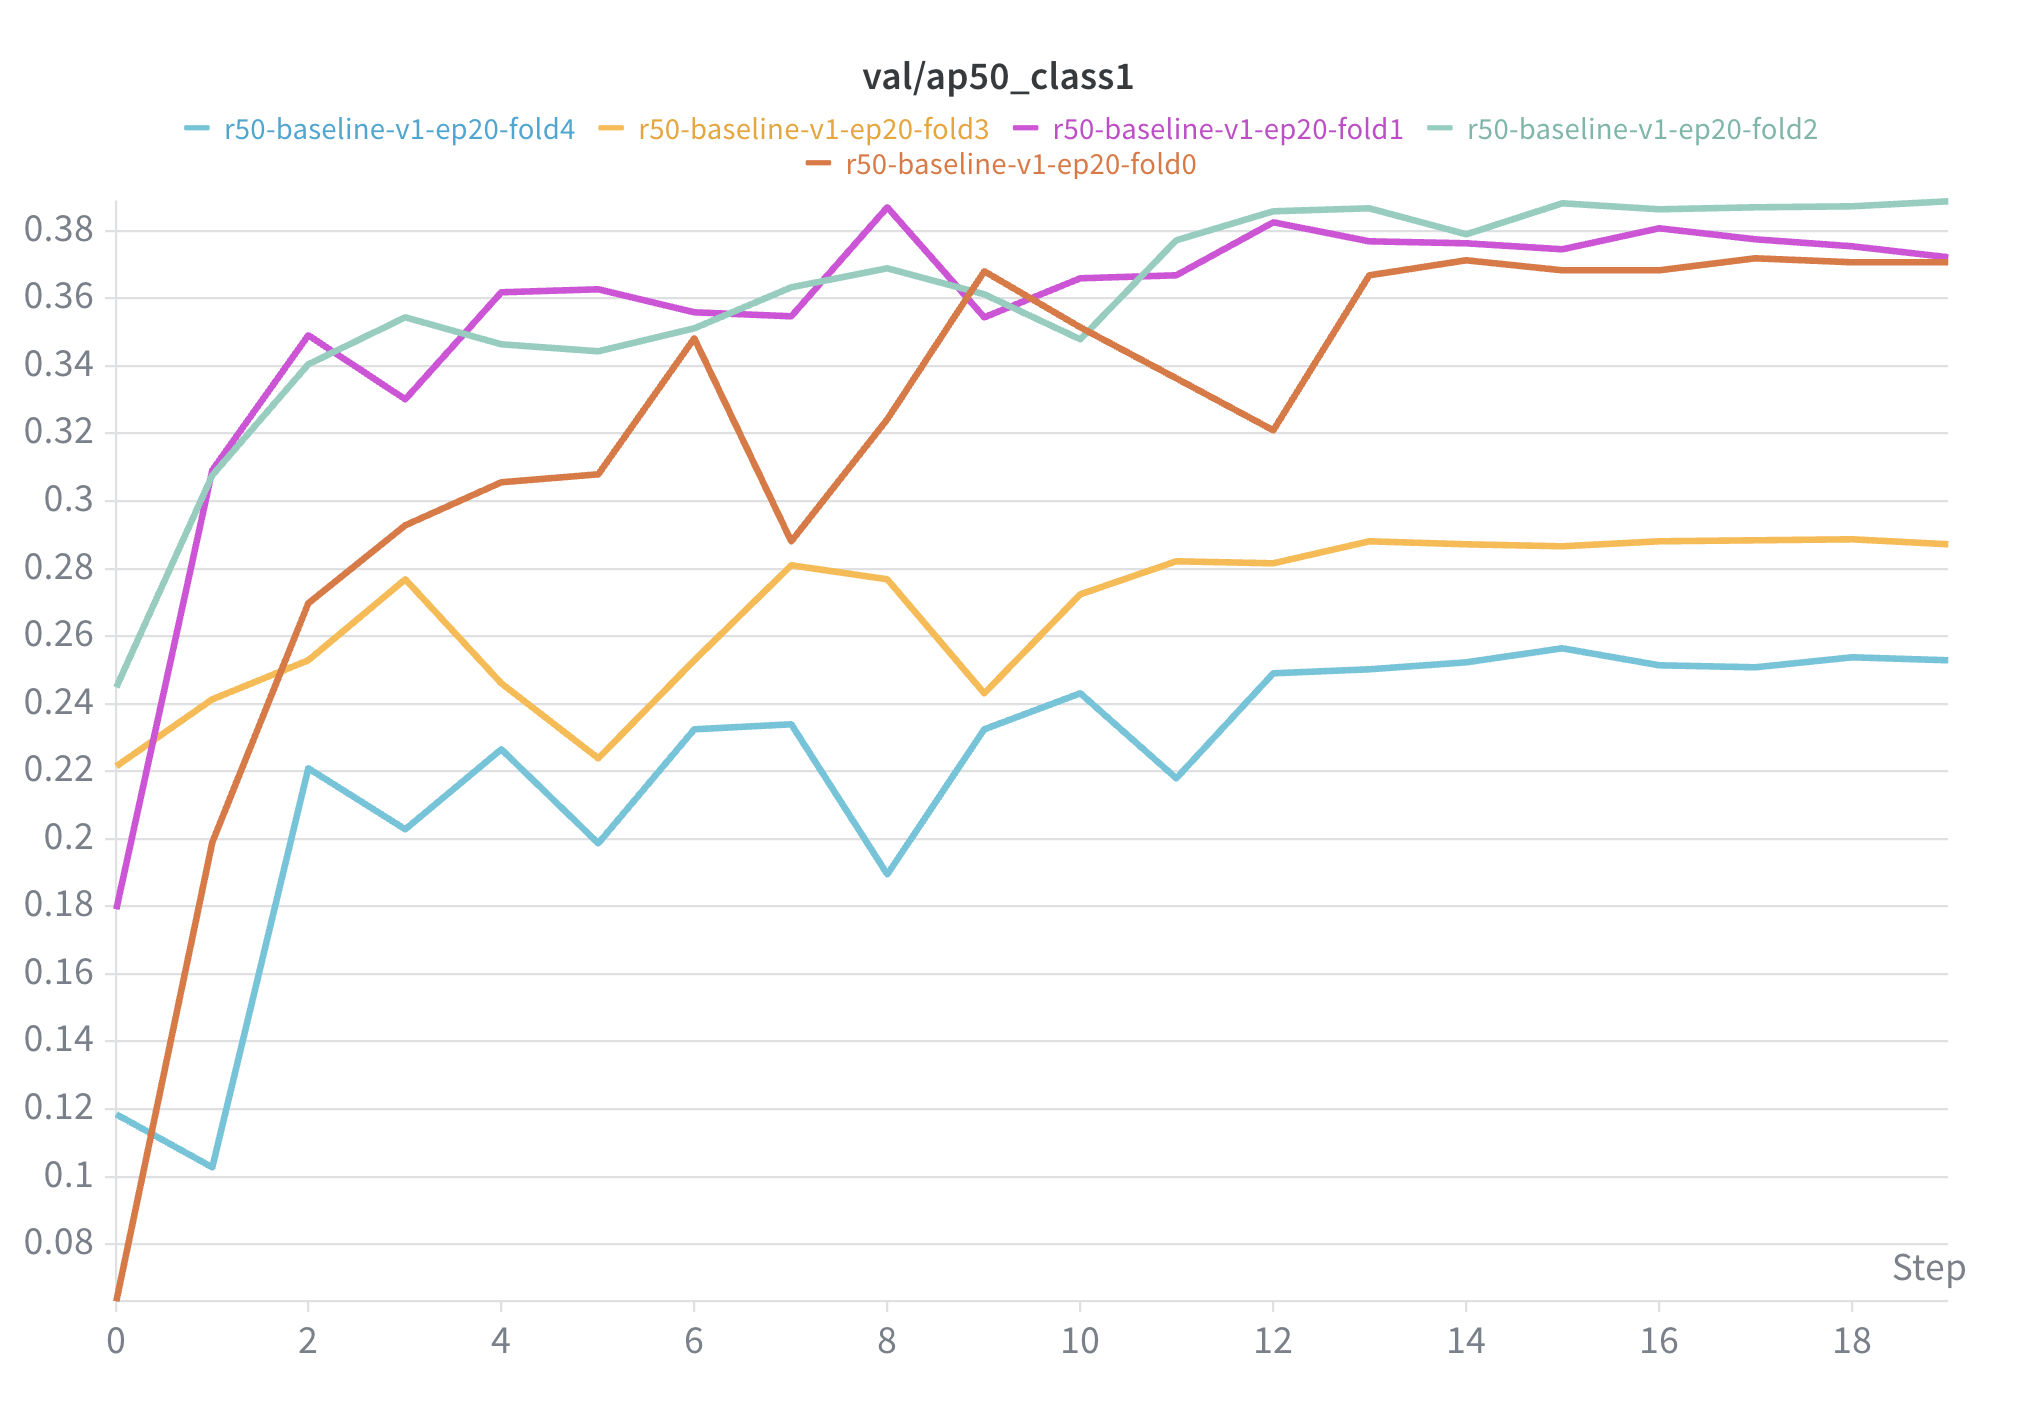
\includegraphics[width=\linewidth]{assets/5-fold/val_ap50_class1.png}
    \caption{Class1: fold2 best.}
  \end{subfigure}

  \vspace{0.5em}
  \begin{subfigure}[t]{0.32\linewidth}
    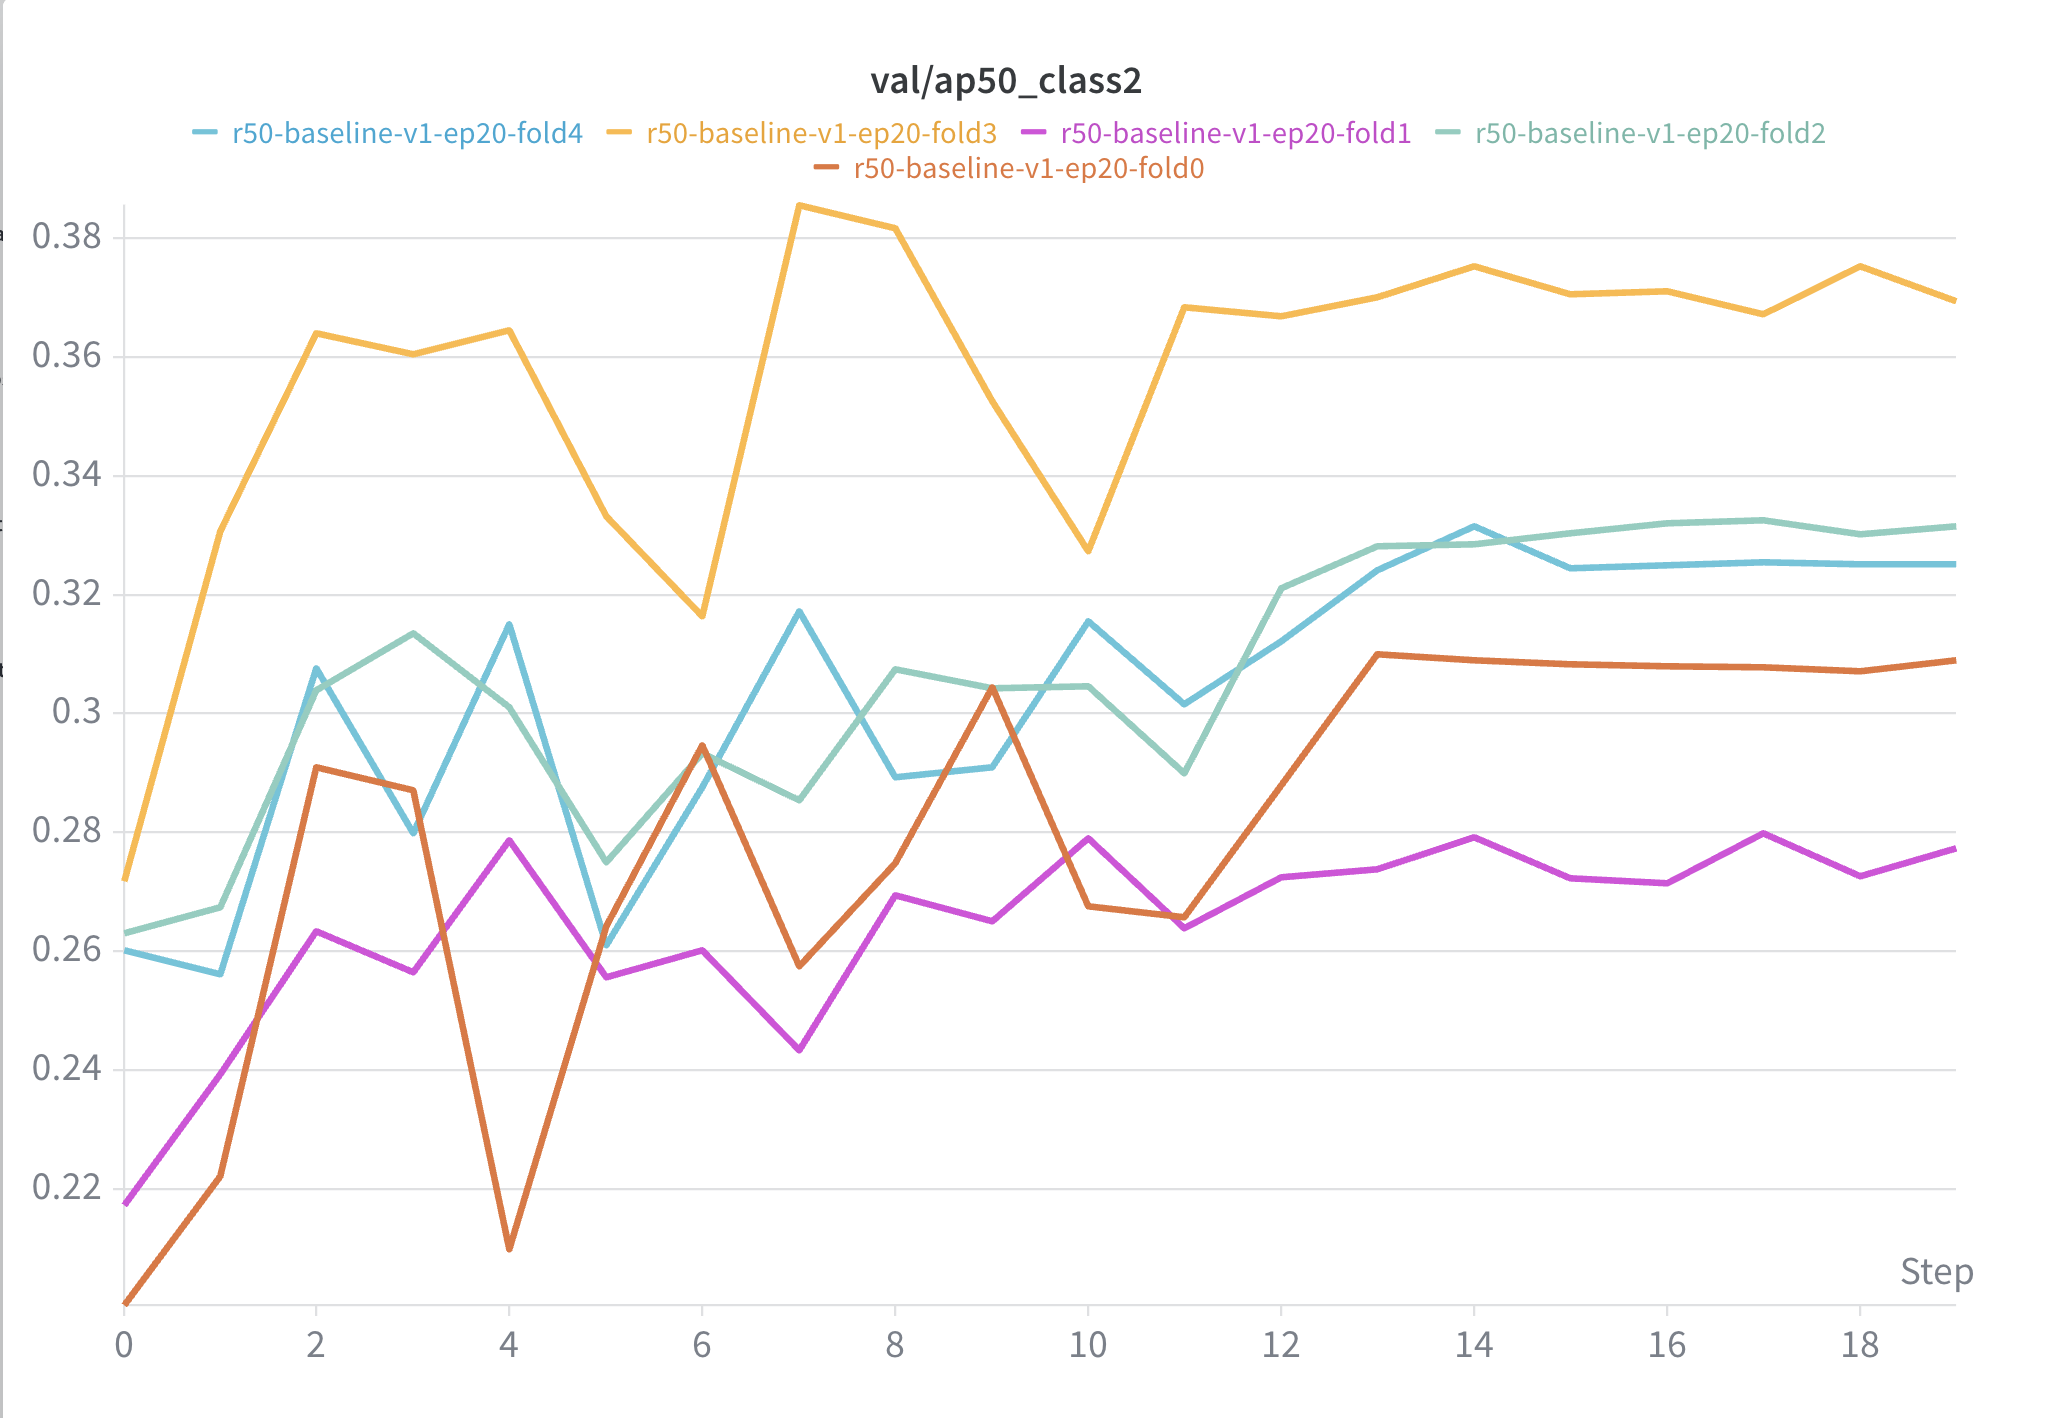
\includegraphics[width=\linewidth]{assets/5-fold/val_ap50_class2.png}
    \caption{Class2: fold3 best.}
  \end{subfigure}
  \hfill
  \begin{subfigure}[t]{0.32\linewidth}
    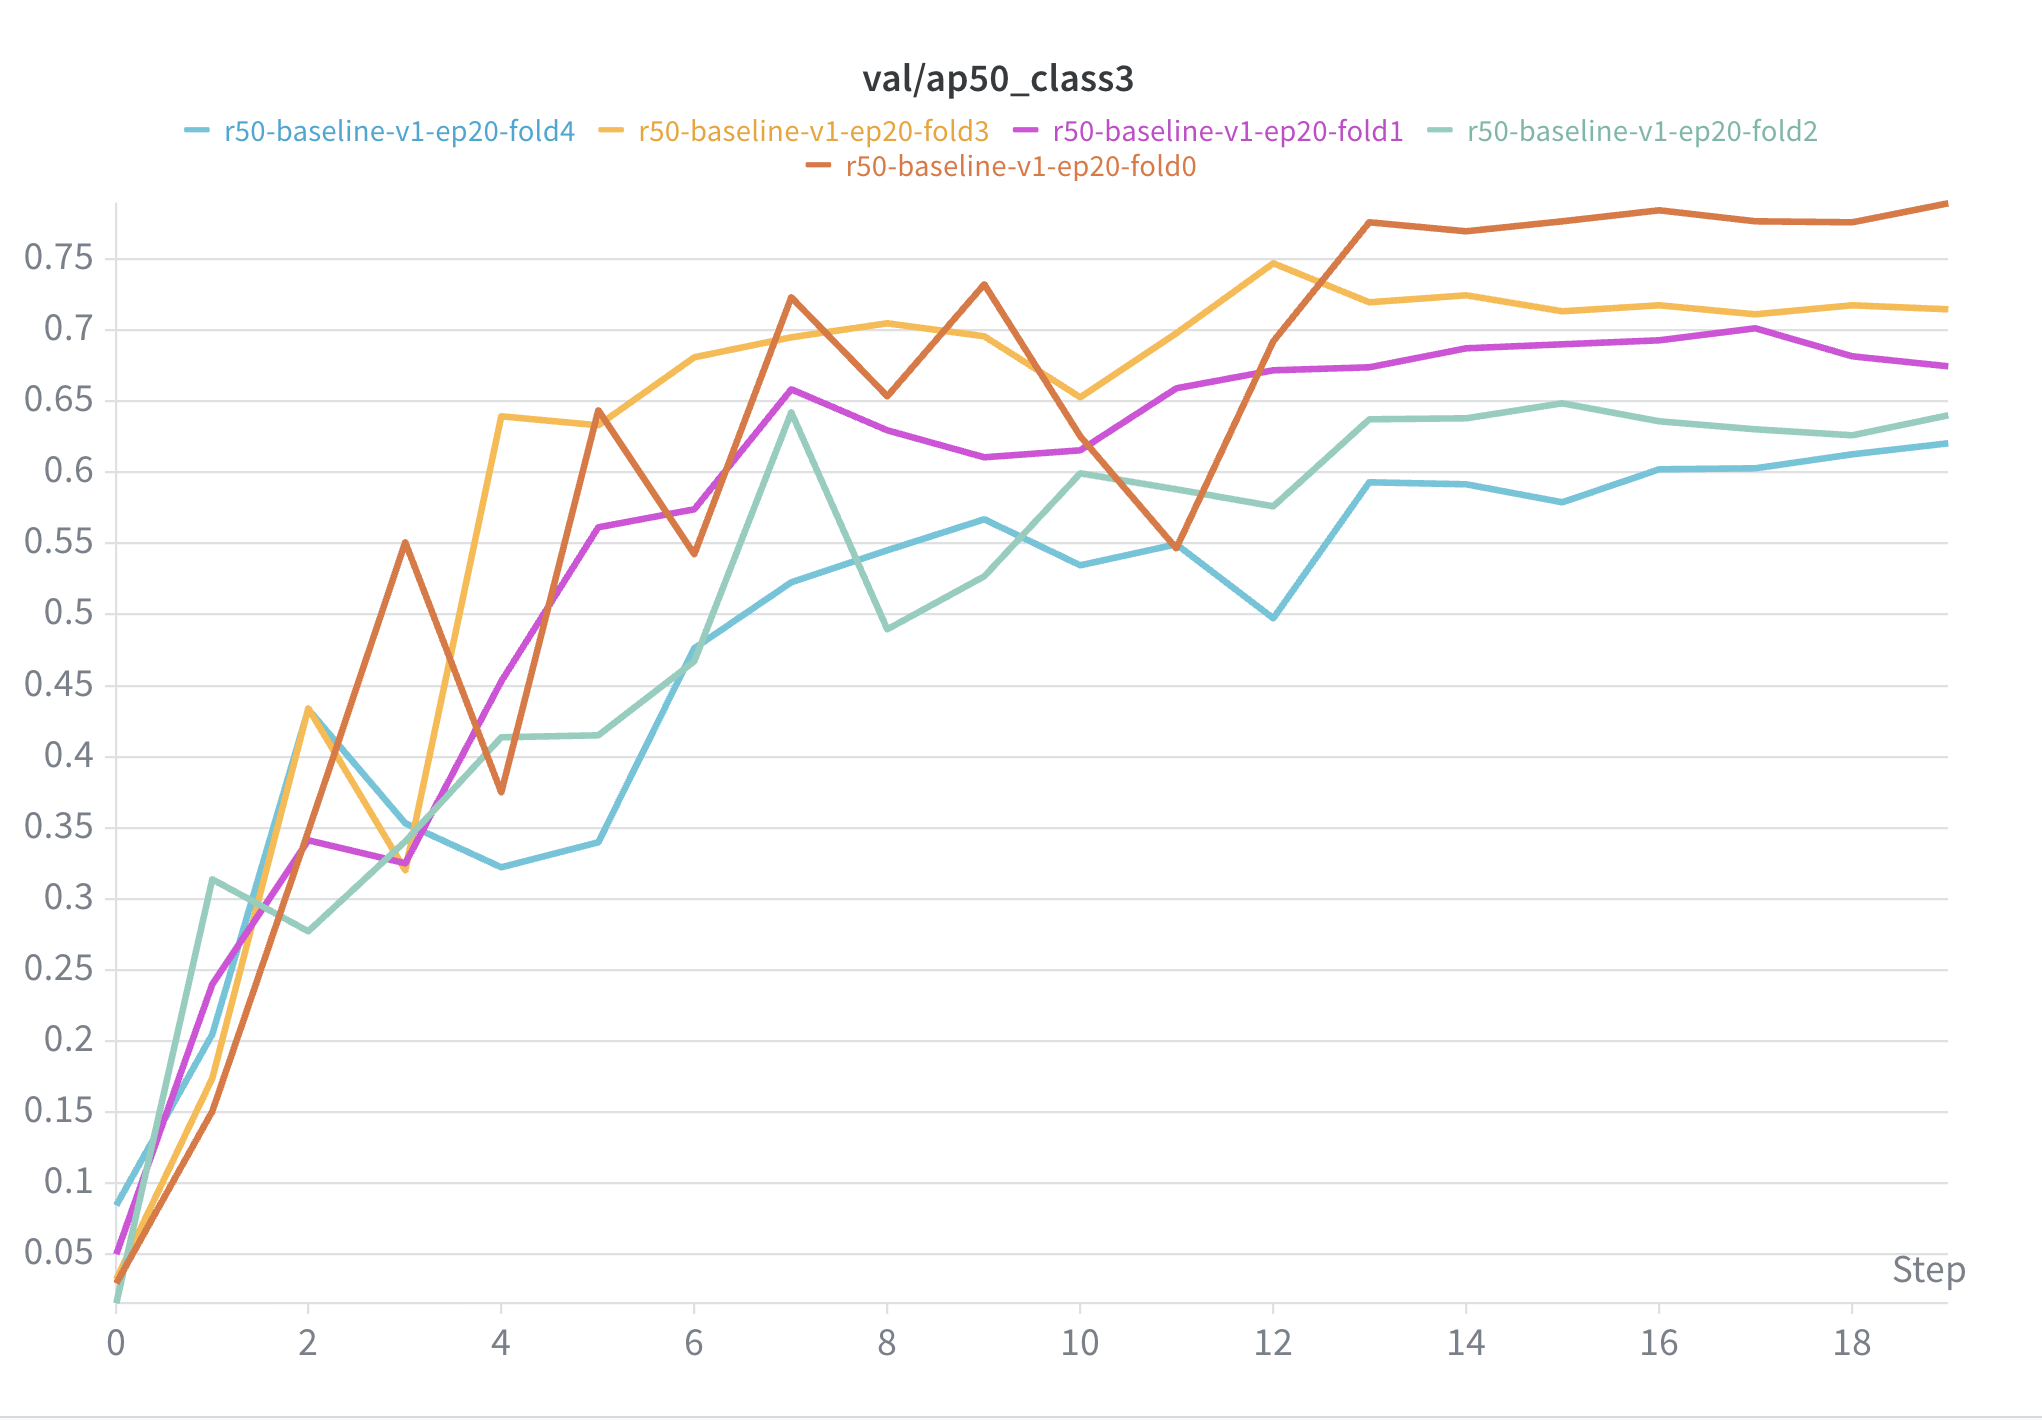
\includegraphics[width=\linewidth]{assets/5-fold/val_ap50_class3.png}
    \caption{Class3: fold0 best.}
  \end{subfigure}
  \hfill
  \begin{subfigure}[t]{0.32\linewidth}
    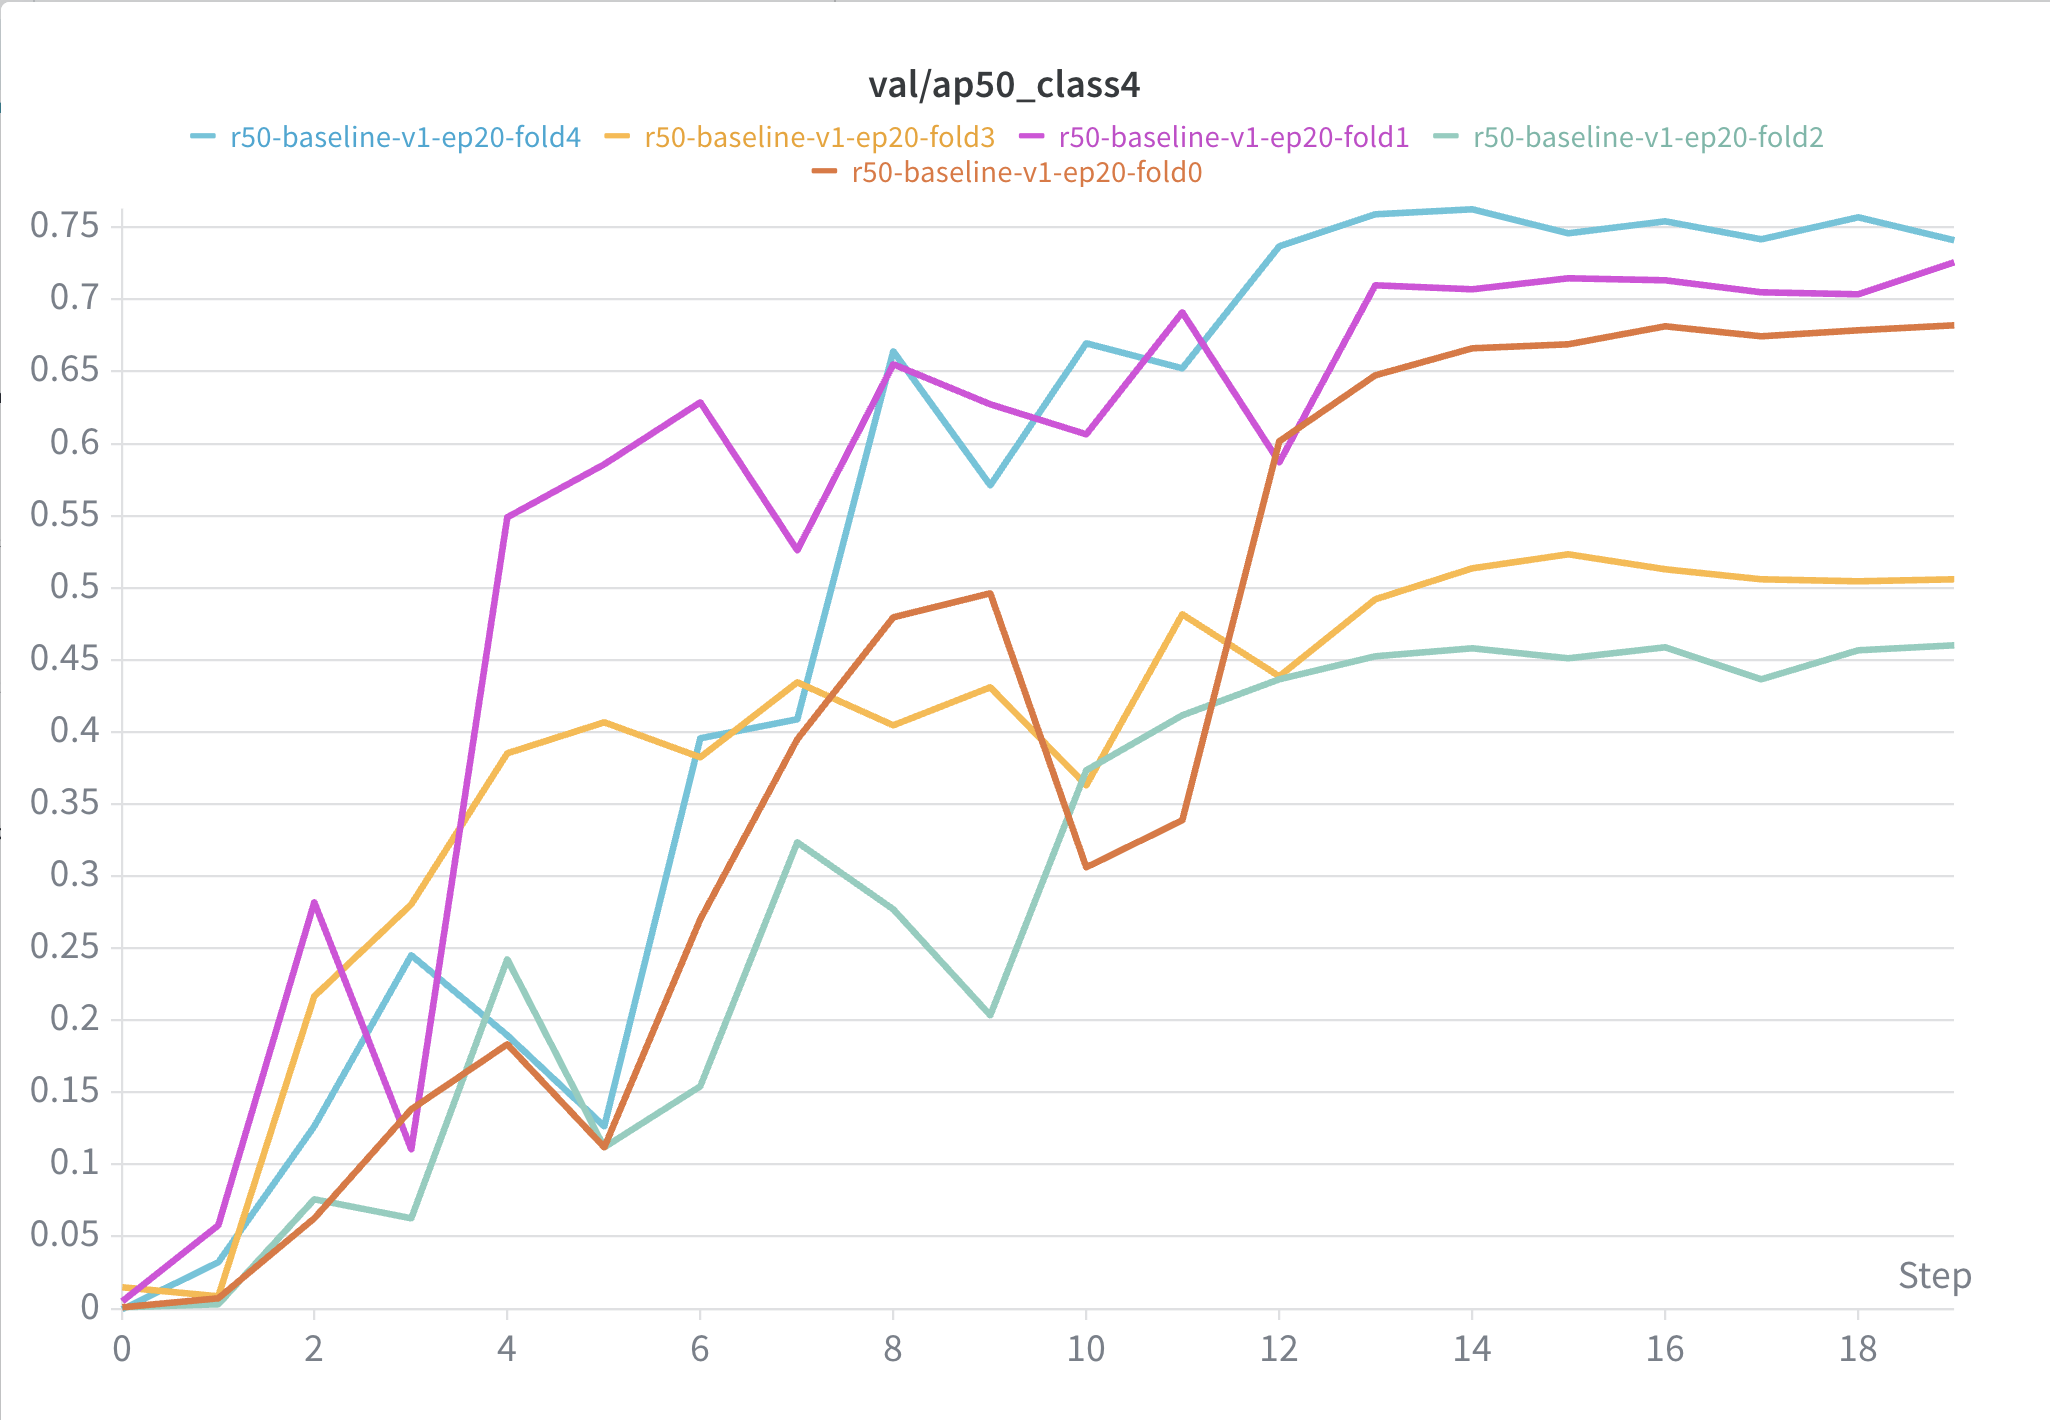
\includegraphics[width=\linewidth]{assets/5-fold/val_ap50_class4.png}
    \caption{Class4: fold4 best.}
  \end{subfigure}
  \caption{5-fold validation curves. Different folds dominate different classes, exposing severe class-wise split sensitivity.}
  \label{fig:fold_curves}
\end{figure*}

\section{Negative Results and Analysis}
\label{sec:negative}

Several theoretically reasonable changes did not improve the public score.

For each additional experiment, we explicitly tracked the hypothesis, expected mechanism, result, and implication, as summarized in \cref{tab:hypotheses}. This was useful because several ideas improved or looked competitive on validation but failed on the public leaderboard.

\begin{table*}[t]
  \centering
  \scriptsize
  \setlength{\tabcolsep}{3pt}
  \begin{tabularx}{\textwidth}{p{0.14\textwidth}X X p{0.18\textwidth} X}
    \toprule
    \textbf{Experiment} & \textbf{Hypothesis} & \textbf{Mechanism} & \textbf{Result} & \textbf{Implication} \\ \midrule
    Multi-scale flip TTA & Test cells have large scale and orientation variation. & Average predictions across flips/scales and fuse masks. & 0.5134 $\rightarrow$ \textbf{0.5624}. & Strongest contribution; improves recall without retraining. \\
    PAFPN neck & Bottom-up path aggregation should improve localization. & Add PANet-style feature aggregation to FPN. & 0.5480, below baseline TTA. & Extra neck capacity did not transfer on 209 images. \\
    Rare-class sampling & More class3/class4 exposure should improve rare-class AP. & Oversample images containing class3 or class4. & 0.5312. & Image-level oversampling caused distribution shift. \\
    Copy-Paste & Synthetic rare instances should improve instance diversity. & Paste class3/class4 masks into training images. & 0.5545 at epoch 30; below best baseline. & Rare-class diversity was not enough to offset context mismatch. \\
    5-fold ensemble & Fold diversity should reduce variance and improve robustness. & Train 5 stratified folds and fuse model/TTA candidates. & 0.5042 direct ensemble. & Weak individual folds and class-specific fold bias hurt ensemble quality. \\
    \bottomrule
  \end{tabularx}
  \caption{Additional experiments beyond hyper-parameter tuning, with hypothesis, mechanism, result, and implication.}
  \label{tab:hypotheses}
\end{table*}

\paragraph{PAFPN.} PAFPN adds a bottom-up path to enrich localization features. However, R50-PAFPN scored 0.5480 with multi-scale TTA, below the R50-FPN baseline. The likely reason is that the dataset has only 209 training images, and the extra neck capacity overfits or changes the feature distribution without improving AP$_{50}$ recall.

\paragraph{Rare-class sampling.} Rare-class weighted sampling was expected to improve class3/class4 recall, but it scored 0.5312. Our implementation is intentionally simple: images containing class3 or class4 are sampled more frequently. This oversamples not only rare cells but also their backgrounds and co-occurring dense class1/class2 contexts, shifting the image distribution away from test data.

\paragraph{Copy-Paste.} Copy-Paste was less harmful than rare-class sampling but still below baseline: 0.5545 at epoch 30 and 0.5410 at epoch 20. It may increase rare-class variety, but the pasted instances can introduce unnatural overlaps and context mismatch. Since public AP$_{50}$ is dominated by dense class1/class2 recall, rare-class gains did not compensate for this distribution shift.

\paragraph{5-fold ensembling.} We trained five baseline-v1 20-epoch folds and tried two ensemble strategies. Post-hoc fusion of already-fused per-fold JSONs scored 0.5078, and direct 5-checkpoint model$\times$TTA fusion scored 0.5042. This shows that ensembling cannot rescue weak individual fold checkpoints. Since fold0 alone scored only 0.4573, the average model quality was much lower than the original baseline checkpoint. The per-class curves also explain why the ensemble was unstable: each fold specialized in different classes, but none was uniformly strong across all four classes. The direct ensemble implementation is conceptually better than JSON-level double fusion, but the input models were not strong enough.

\section{Conclusion}
\label{sec:conclusion}

The final system uses TorchVision Mask R-CNN with ResNet-50-FPN, small anchors, high detection cap, strong geometric/color augmentation, and streaming multi-scale flip TTA. The best public AP$_{50}$ is \textbf{0.5624}, well above the strong baseline threshold. The main lesson is that, for this small dense-cell dataset, robust inference-time augmentation and memory-safe mask fusion were more valuable than heavier necks, rare-class oversampling, or naive k-fold ensembling.

GitHub repository: \url{https://github.com/ChuEating1005/VRDL/tree/main/HW3}.

{\small
  \bibliographystyle{ieee_fullname}
  \bibliography{egbib}
}

\end{document}
